\documentclass[12pt,a4paper]{article}

% ============================================
% PACKAGES
% ============================================
\usepackage{fontspec}
\usepackage{unicode-math}
\usepackage[vietnamese]{babel}
\usepackage{geometry}
\usepackage{graphicx}
\usepackage{amsmath}
\usepackage{amssymb}
\usepackage{xcolor}
\usepackage{hyperref}
\usepackage{float}
\usepackage{caption}
\usepackage{subcaption}
\usepackage{booktabs}
\usepackage{tikz}
\usetikzlibrary{positioning}

% ============================================
% FONT SETTINGS
% ============================================
\setmainfont{Libertinus Serif}
\setmathfont{Libertinus Math}

% ============================================
% PAGE LAYOUT
% ============================================
\geometry{
    left=2.5cm,
    right=2.5cm,
    top=2.5cm,
    bottom=2.5cm
}

% ============================================
% COLORS
% ============================================
\definecolor{backcolour}{rgb}{0.95,0.95,0.92}

% ============================================
% HYPERLINK SETTINGS
% ============================================
\hypersetup{
    colorlinks=true,
    linkcolor=blue!50!black,
    urlcolor=blue!50!black,
    citecolor=blue!50!black,
    pdftitle={Bao cao Mini-project Lab 09},
    pdfauthor={Bui Quang Chien}
}

\setcounter{tocdepth}{2}
\setcounter{secnumdepth}{3}

\begin{document}

% ============================================
% TITLE PAGE
% ============================================
\begin{titlepage}
    \centering
    \vspace*{2cm}

    {\LARGE\bfseries TRƯỜNG ĐẠI HỌC KHOA HỌC TỰ NHIÊN\\[0.3cm]
    KHOA TOÁN - CƠ - TIN HỌC\\[0.5cm]}

    \begin{figure}[H]
        \centering
        \IfFileExists{../../../../../LOGOHUS.png}{
            \includegraphics[width=0.3\linewidth]{../../../../../LOGOHUS.png}
        }{
            \IfFileExists{../../../../../LOGOHUS.jpg}{
                \includegraphics[width=0.3\linewidth]{../../../../../LOGOHUS.jpg}
            }{
                \fbox{LOGO HUS}
            }
        }
    \end{figure}

    {\huge\bfseries BÁO CÁO MINI-PROJECT\\[0.5cm]
    MÔN: THỊ GIÁC MÁY TÍNH (MAT3562E 2)\\[0.5cm]}

    {\Large\bfseries LAB 09: KHÔNG GIAN MÀU TRONG XỬ LÝ ẢNH\\[0.3cm]
    HỆ THỐNG PHÁT HIỆN ĐỐI TƯỢNG THEO MÀU\\[1.5cm]}

    \begin{flushleft}
    {\large
    Giảng viên: TS. Cao Văn Chung\\
    Sinh viên: Bùi Quang Chiến\\
    MSSV: 23001837\\
    Lớp: MAT3562E 2\\
    }
    \end{flushleft}

    \vfill

    {\large Hà Nội, tháng 4 năm 2026}
\end{titlepage}

\tableofcontents
\newpage

% ============================================
% NỘI DUNG BÁO CÁO
% ============================================

\section{Mục tiêu và phạm vi báo cáo}

Báo cáo này tổng hợp phần thực hành trọng tâm của Lab 09 trên notebook
\texttt{lab09\_BuiQuangChien\_23001837.ipynb}, gồm:
\begin{itemize}
    \item Bài toán 4: dò biên theo Gray, kênh $Y$ trong XYZ, gradient véc-tơ XYZ, gradient véc-tơ Lab.
    \item Bài toán 5: phân đoạn K-means trong XYZ và Lab, có mở rộng thêm đặc trưng không gian $(x, y)$.
    \item Phần bắt buộc: bộ ảnh synthetic minh họa failure modes.
    \item Mini-project: phát hiện đối tượng màu theo hai phương án đối chứng (XYZ-$Y$ và khoảng cách Lab).
\end{itemize}

\section{Dữ liệu và thiết lập thực nghiệm}

\subsection{Bài toán mini-project}
Mục tiêu mini-project là phát hiện trái cây có màu nổi bật trong ảnh ngoài trời bằng hai pipeline:
\begin{enumerate}
    \item Pipeline A: ngưỡng trên kênh $Y$ trong không gian XYZ.
    \item Pipeline B: ngưỡng theo khoảng cách màu trong không gian Lab.
\end{enumerate}

\subsection{Bộ ảnh sử dụng}
Tập mini-project sử dụng 5 ảnh trong nhóm \texttt{fruit}:
\texttt{fruit1.png}, \texttt{fruit2 (1).jpg}, \texttt{fruit2.jpg}, \texttt{fruit3.png}, \texttt{fruit4.png}.

\subsection{Các tham số chính}
\begin{itemize}
    \item Chuẩn hóa kích thước ảnh: \texttt{max\_side = 320}.
    \item Pipeline A (XYZ-$Y$): dùng ngưỡng theo quantile $q_Y = 0.62$.
    \item Pipeline B (Lab): dùng ngưỡng theo quantile khoảng cách màu $q_{Lab} = 0.28$.
    \item Hậu xử lý hình thái học: Opening + Closing với kernel $5\times5$.
    \item Lọc contour theo diện tích tối thiểu: $A_{\min}=200\,\text{pixels}^2$.
\end{itemize}

\subsection{Công thức sử dụng}
\begin{align}
\text{Pipeline A: } & M_Y(x,y)=\mathbb{1}\{Y(x,y)\ge T_Y\} \\
\text{Pipeline B: } & d_{Lab}(x,y)=\sqrt{(L-L_0)^2+(a-a_0)^2+(b-b_0)^2},\quad
M_{Lab}(x,y)=\mathbb{1}\{d_{Lab}(x,y)\le T_{Lab}\}.
\end{align}

\section{Sơ đồ pipeline mini-project}

\begin{figure}[H]
    \centering
    \begin{tikzpicture}[
        node distance=1.5cm,
        every node/.style={
            draw,
            rectangle,
            fill=backcolour,
            align=center,
            rounded corners,
            minimum width=3.3cm,
            minimum height=1cm
        }
    ]
        \node (input) {Ảnh gốc RGB};

        \node (xyz) [below left=1.5cm and 2.0cm of input] {RGB $\to$ XYZ\\Lấy kênh $Y$};
        \node (lab) [below right=1.5cm and 2.0cm of input] {RGB $\to$ XYZ $\to$ Lab\\Tính $d_{Lab}$ tới màu đích};

        \node (thrA) [below=0.7cm of xyz] {Ngưỡng $Y\ge T_Y$};
        \node (thrB) [below=0.7cm of lab] {Ngưỡng $d_{Lab}\le T_{Lab}$};

        \node (morphA) [below=0.7cm of thrA] {Opening + Closing};
        \node (morphB) [below=0.7cm of thrB] {Opening + Closing};

        \node (contourA) [below=0.7cm of morphA] {Contour + lọc diện tích\\Bounding box};
        \node (contourB) [below=0.7cm of morphB] {Contour + lọc diện tích\\Bounding box};

        \node (outA) [below=0.7cm of contourA] {Kết quả A};
        \node (outB) [below=0.7cm of contourB] {Kết quả B};

        \draw[->, thick] (input) -- (xyz);
        \draw[->, thick] (input) -- (lab);
        \draw[->, thick] (xyz) -- (thrA);
        \draw[->, thick] (lab) -- (thrB);
        \draw[->, thick] (thrA) -- (morphA);
        \draw[->, thick] (thrB) -- (morphB);
        \draw[->, thick] (morphA) -- (contourA);
        \draw[->, thick] (morphB) -- (contourB);
        \draw[->, thick] (contourA) -- (outA);
        \draw[->, thick] (contourB) -- (outB);
    \end{tikzpicture}
    \caption{Pipeline phát hiện đối tượng màu: XYZ-$Y$ đối chứng với Lab-distance}
    \label{fig:pipeline}
\end{figure}

\section{Kết quả Bài toán 4: Dò biên}

\subsection{Kết quả định tính}
Notebook đã sinh đầy đủ ảnh so sánh gradient và contour cho 8 ảnh thật
(2 ảnh mỗi nhóm: outdoor, multicolors, shadow, fruit), cùng bộ ảnh synthetic.

\begin{figure}[H]
    \centering
    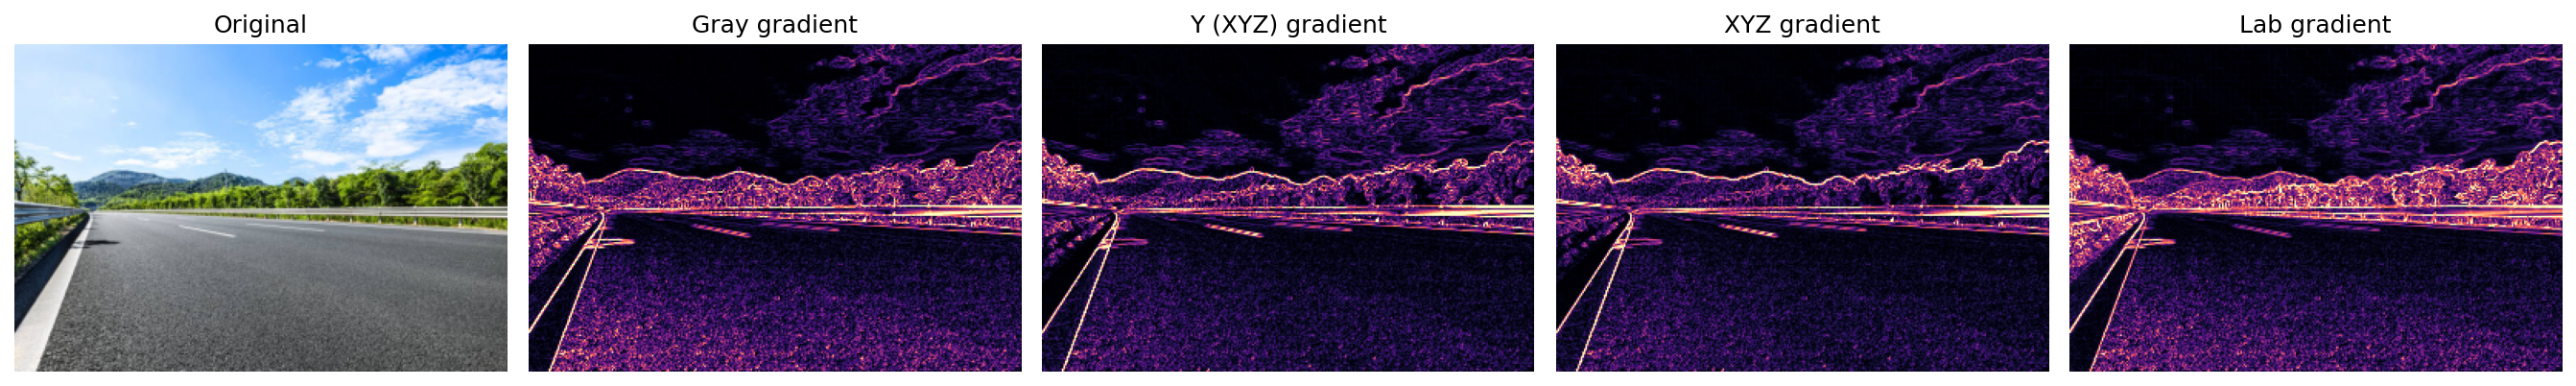
\includegraphics[width=0.95\linewidth]{outputs/problem4_outdoor_outdoor1_gradients.png}
    \caption{Ví dụ so sánh bản đồ gradient 4 phương pháp trên ảnh outdoor1}
\end{figure}

\begin{figure}[H]
    \centering
    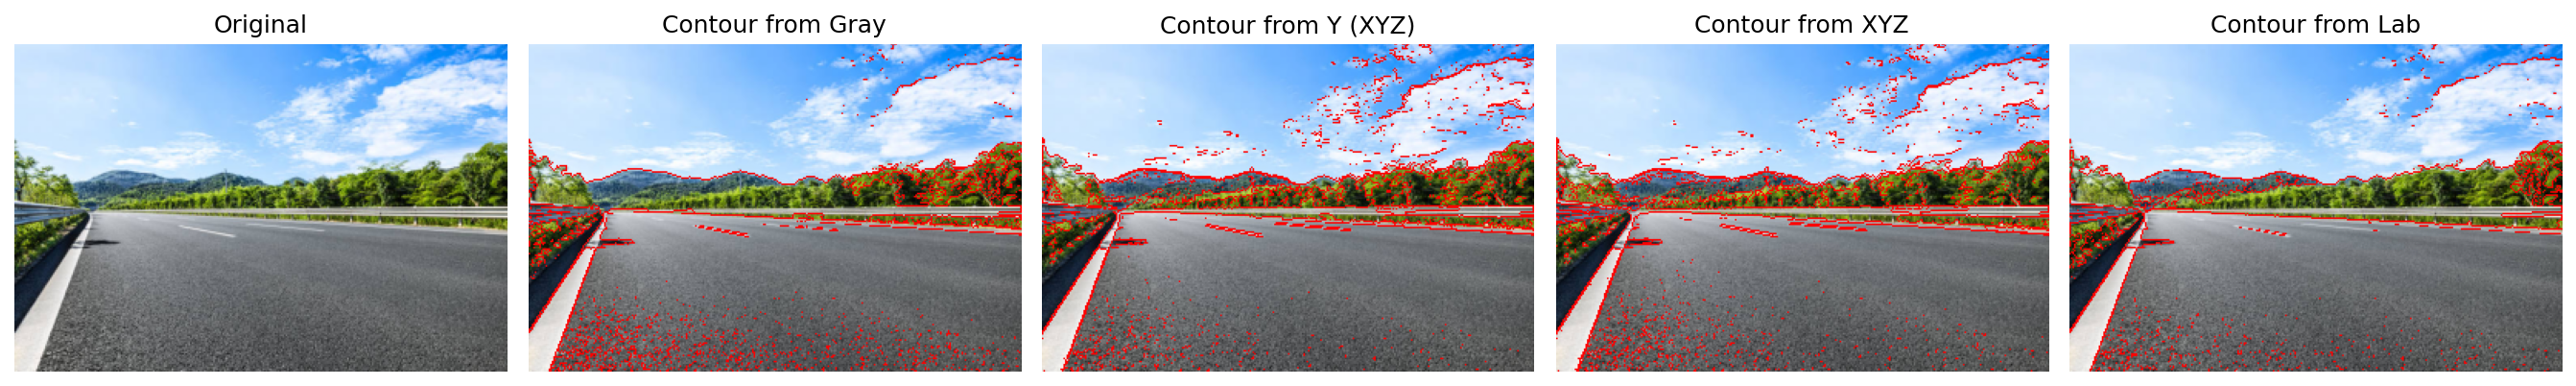
\includegraphics[width=0.95\linewidth]{outputs/problem4_outdoor_outdoor1_contours.png}
    \caption{Ví dụ so sánh contour trích xuất từ 4 phương pháp trên ảnh outdoor1}
\end{figure}

\subsection{Tóm tắt định lượng từ \texttt{problem4\_edge\_metrics.csv}}
\begin{table}[H]
    \centering
    \caption{Giá trị trung bình theo phương pháp (8 ảnh thật)}
    \begin{tabular}{lcc}
        \toprule
        Phương pháp & Contour trung bình & Edge ratio trung bình \\
        \midrule
        Gray & 572.38 & 0.1000 \\
        Y (XYZ) & 506.63 & 0.1000 \\
        XYZ (vector) & 514.88 & 0.1000 \\
        Lab (vector) & 475.63 & 0.1000 \\
        \bottomrule
    \end{tabular}
\end{table}

Do cùng quy tắc ngưỡng theo quantile ($q=0.90$), edge ratio gần như cố định quanh $0.1$.
Sự khác biệt chính thể hiện qua hình thái contour và mức độ phân mảnh giữa các hệ màu.

\section{Phần minh họa trực quan bắt buộc với ảnh synthetic}

\subsection{Isoluminant boundary}
\subsubsection{Ý tưởng thiết kế}
Hai nửa ảnh có màu khác nhau nhưng giữ mức sáng gần tương đương.

\subsubsection{Dự đoán trước khi chạy}
Gray và $Y$ sẽ khó phát hiện biên rõ, còn XYZ/Lab gradient sẽ thể hiện biên màu tốt hơn.

\subsubsection{Quan sát sau khi chạy}
Biên màu trong XYZ/Lab nổi bật hơn Gray, đúng với kỳ vọng về failure mode isoluminant.

\begin{figure}[H]
    \centering
    \begin{subfigure}{0.48\linewidth}
        \centering
        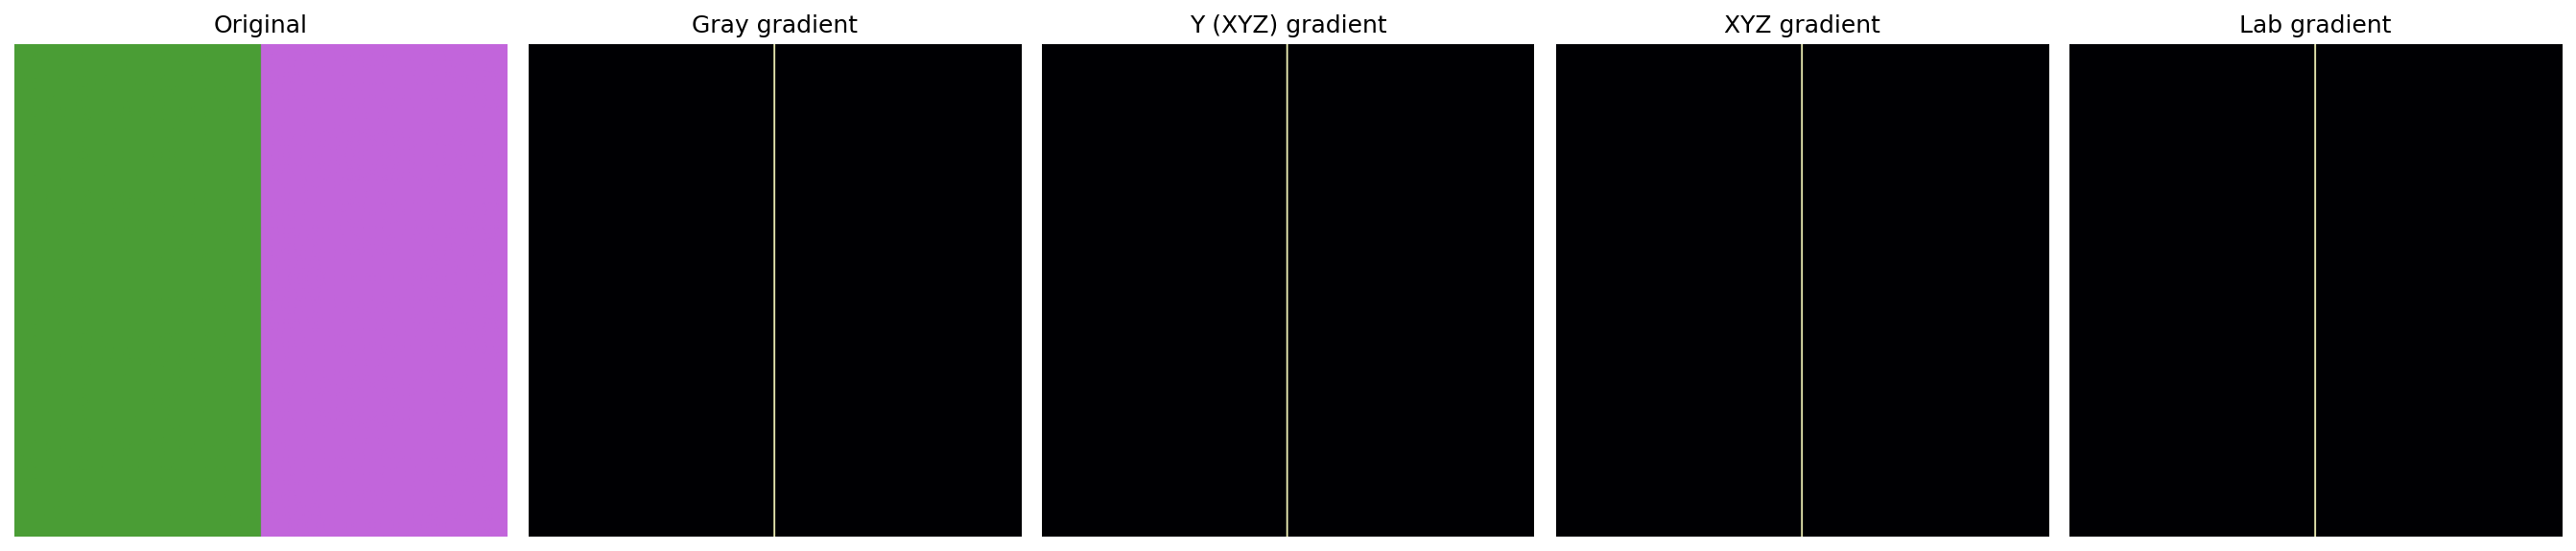
\includegraphics[width=\linewidth]{outputs/synthetic_isoluminant_boundary_gradients.png}
        \caption{Gradient maps}
    \end{subfigure}
    \hfill
    \begin{subfigure}{0.48\linewidth}
        \centering
        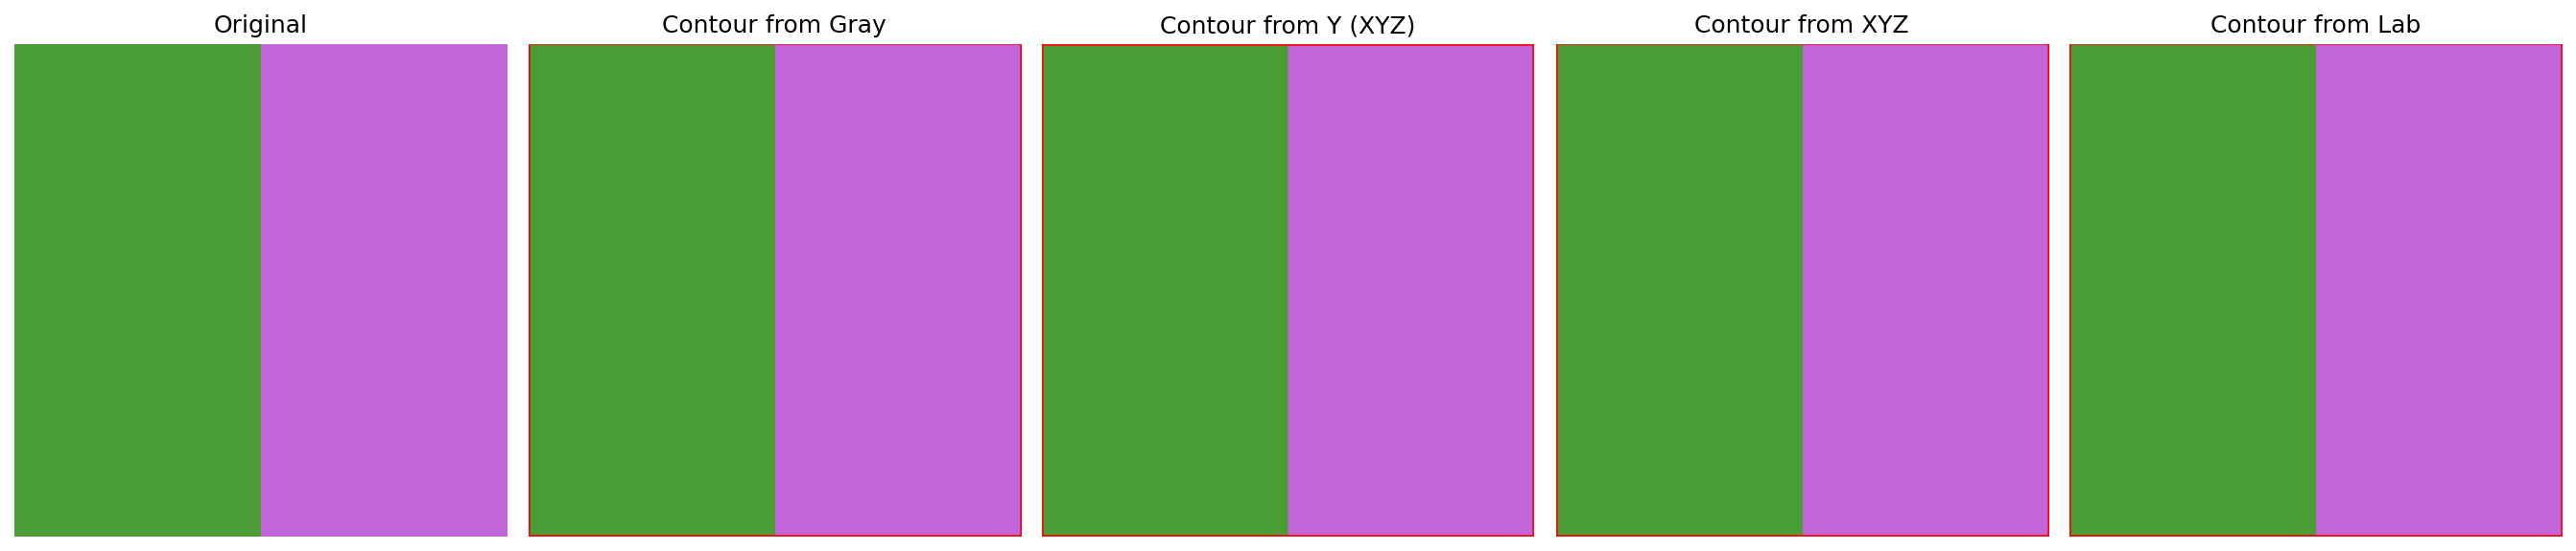
\includegraphics[width=\linewidth]{outputs/synthetic_isoluminant_boundary_contours.png}
        \caption{Contours}
    \end{subfigure}
    \caption{Synthetic 1: isoluminant boundary}
\end{figure}

\subsection{Chromatic texture}
\subsubsection{Ý tưởng thiết kế}
Checkerboard hai màu có độ chói gần nhau để gây nhiễu với phương pháp dựa sáng.

\subsubsection{Dự đoán trước khi chạy}
Phương pháp dựa $Y$ có nguy cơ bỏ sót hoặc không ổn định, trong khi gradient màu hoạt động tốt hơn.

\subsubsection{Quan sát sau khi chạy}
Các biên cấu trúc màu xuất hiện rõ trong không gian màu, phù hợp với thiết kế dữ liệu.

\subsection{Illumination gradient}
\subsubsection{Ý tưởng thiết kế}
Một nền màu có gradient chiếu sáng mạnh theo trục ngang.

\subsubsection{Dự đoán trước khi chạy}
Phương pháp theo độ sáng sẽ dễ tạo biên giả do thay đổi illumination.

\subsubsection{Quan sát sau khi chạy}
Biên giả do thay đổi sáng được quan sát rõ hơn trong các phương pháp nhạy cường độ.

\subsection{Hidden shape}
\subsubsection{Ý tưởng thiết kế}
Vật thể và nền gần mức sáng nhưng khác sắc độ.

\subsubsection{Dự đoán trước khi chạy}
Gray và $Y$ dễ bỏ sót hình ẩn; gradient Lab có lợi thế nhờ đo chênh màu theo cảm nhận.

\subsubsection{Quan sát sau khi chạy}
Biên vật thể ẩn thể hiện rõ hơn ở không gian màu, nhất là Lab.

\section{Mini-project: 3 ví dụ thành công và 2 ví dụ khó}

\subsection{Bảng kết quả trên 5 ảnh fruit}
\begin{table}[H]
    \centering
    \caption{Kết quả định lượng mini-project từ \texttt{mini\_project\_xyzY\_vs\_lab\_metrics.csv}}
    \begin{tabular}{lcccc}
        \toprule
        Ảnh & Y boxes & Lab boxes & Y mask ratio & Lab mask ratio \\
        \midrule
        fruit1.png & 4 & 7 & 0.3332 & 0.2135 \\
        fruit2 (1).jpg & 15 & 9 & 0.3213 & 0.1244 \\
        fruit2.jpg & 15 & 9 & 0.3213 & 0.1244 \\
        fruit3.png & 14 & 8 & 0.3666 & 0.2391 \\
        fruit4.png & 5 & 8 & 0.3636 & 0.2002 \\
        \bottomrule
    \end{tabular}
\end{table}

\subsection{Ba ví dụ thành công}

\subsubsection{Ca 1: fruit2.jpg}
Lab giảm số box từ 15 xuống 9 (giảm khoảng 40\%), kết quả gọn và ít nhiễu hơn Y.

\subsubsection{Ca 2: fruit3.png}
Lab giảm số box từ 14 xuống 8 (giảm khoảng 42.9\%), tách nền sáng tốt hơn.

\subsubsection{Ca 3: fruit2 (1).jpg}
Ở ảnh biến thể cùng cảnh, xu hướng vẫn giữ nguyên: Lab cho số box thấp hơn Y
(9 so với 15), cho thấy tính ổn định theo cùng kiểu dữ liệu.

\begin{figure}[H]
    \centering
    \begin{subfigure}{0.32\linewidth}
        \centering
        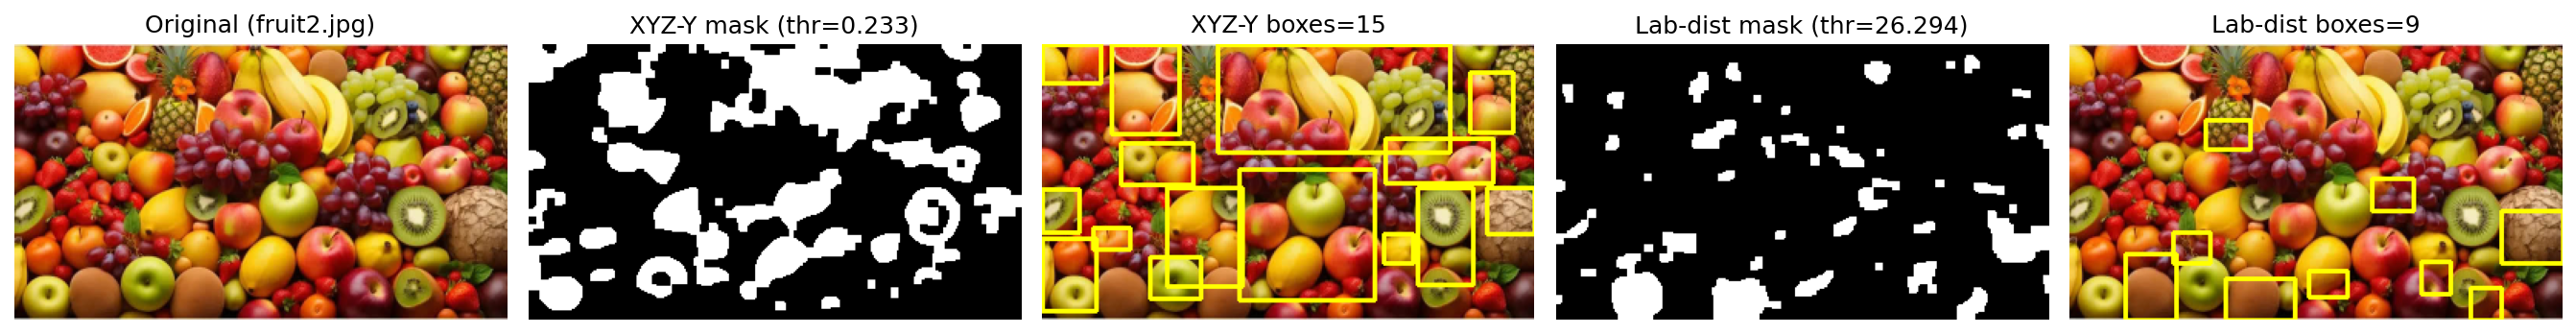
\includegraphics[width=\linewidth]{outputs/mini_project_fruit2_xyzY_vs_lab.png}
        \caption{fruit2.jpg}
    \end{subfigure}
    \hfill
    \begin{subfigure}{0.32\linewidth}
        \centering
        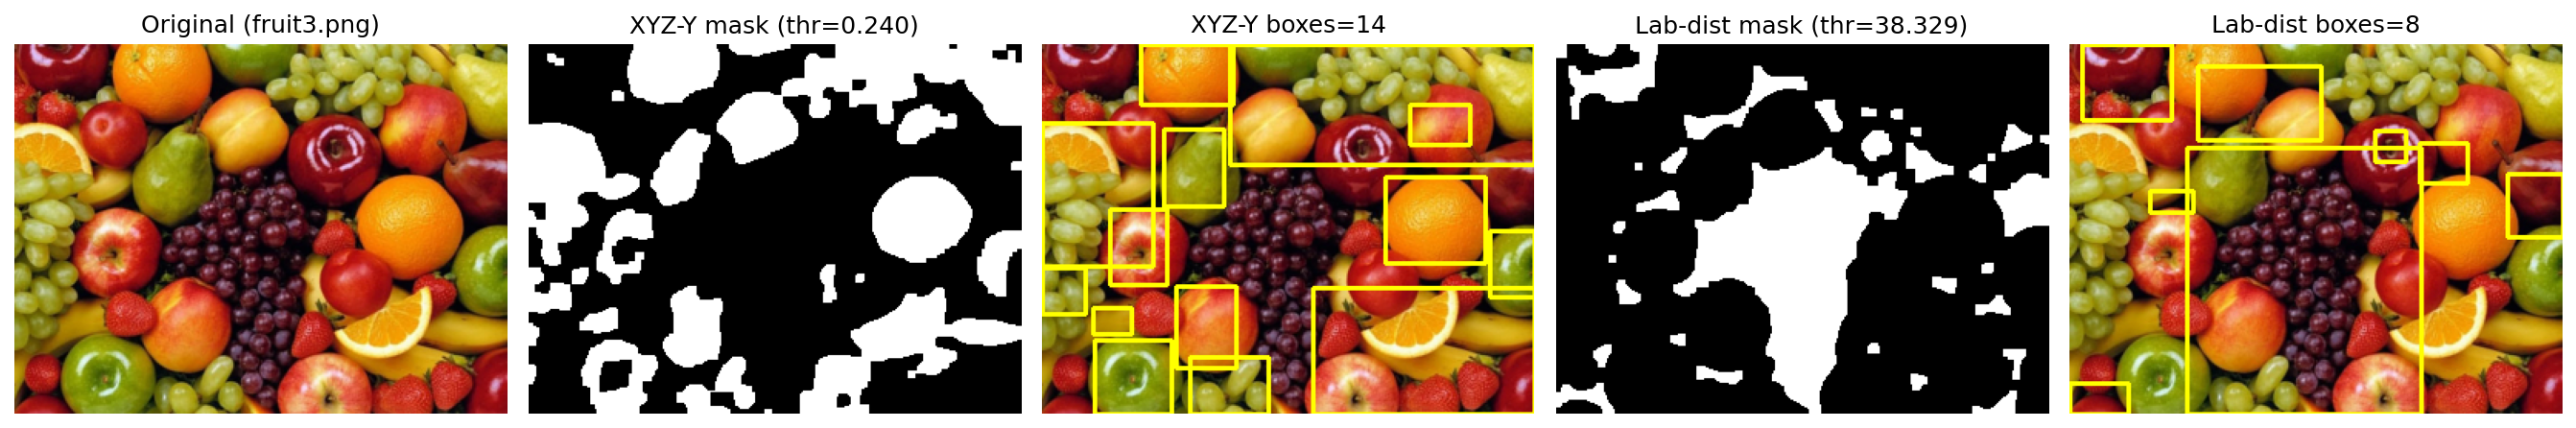
\includegraphics[width=\linewidth]{outputs/mini_project_fruit3_xyzY_vs_lab.png}
        \caption{fruit3.png}
    \end{subfigure}
    \hfill
    \begin{subfigure}{0.32\linewidth}
        \centering
        
\includegraphics[width=\linewidth]{\detokenize{outputs/mini_project_fruit2_(1)_xyzY_vs_lab.png}}
        \caption{fruit2 (1).jpg}
    \end{subfigure}
    \caption{Ba ví dụ thành công của mini-project}
\end{figure}

\subsection{Hai ví dụ khó/thất bại tương đối}

\subsubsection{Ca khó 1: fruit1.png}
Y cho 4 box, Lab cho 7 box. Trường hợp này Lab bị phân mảnh nhiều hơn,
cho thấy khi màu mục tiêu và nền có phân bố gần nhau theo mẫu chọn,
threshold theo $d_{Lab}$ có thể tạo thêm vùng nhiễu.

\subsubsection{Ca khó 2: fruit4.png}
Y cho 5 box, Lab cho 8 box. Đây là ca khó với cả hai phương án;
Lab vẫn giữ mask gọn hơn về diện tích nhưng số box tách rời lại tăng.

\begin{figure}[H]
    \centering
    \begin{subfigure}{0.48\linewidth}
        \centering
        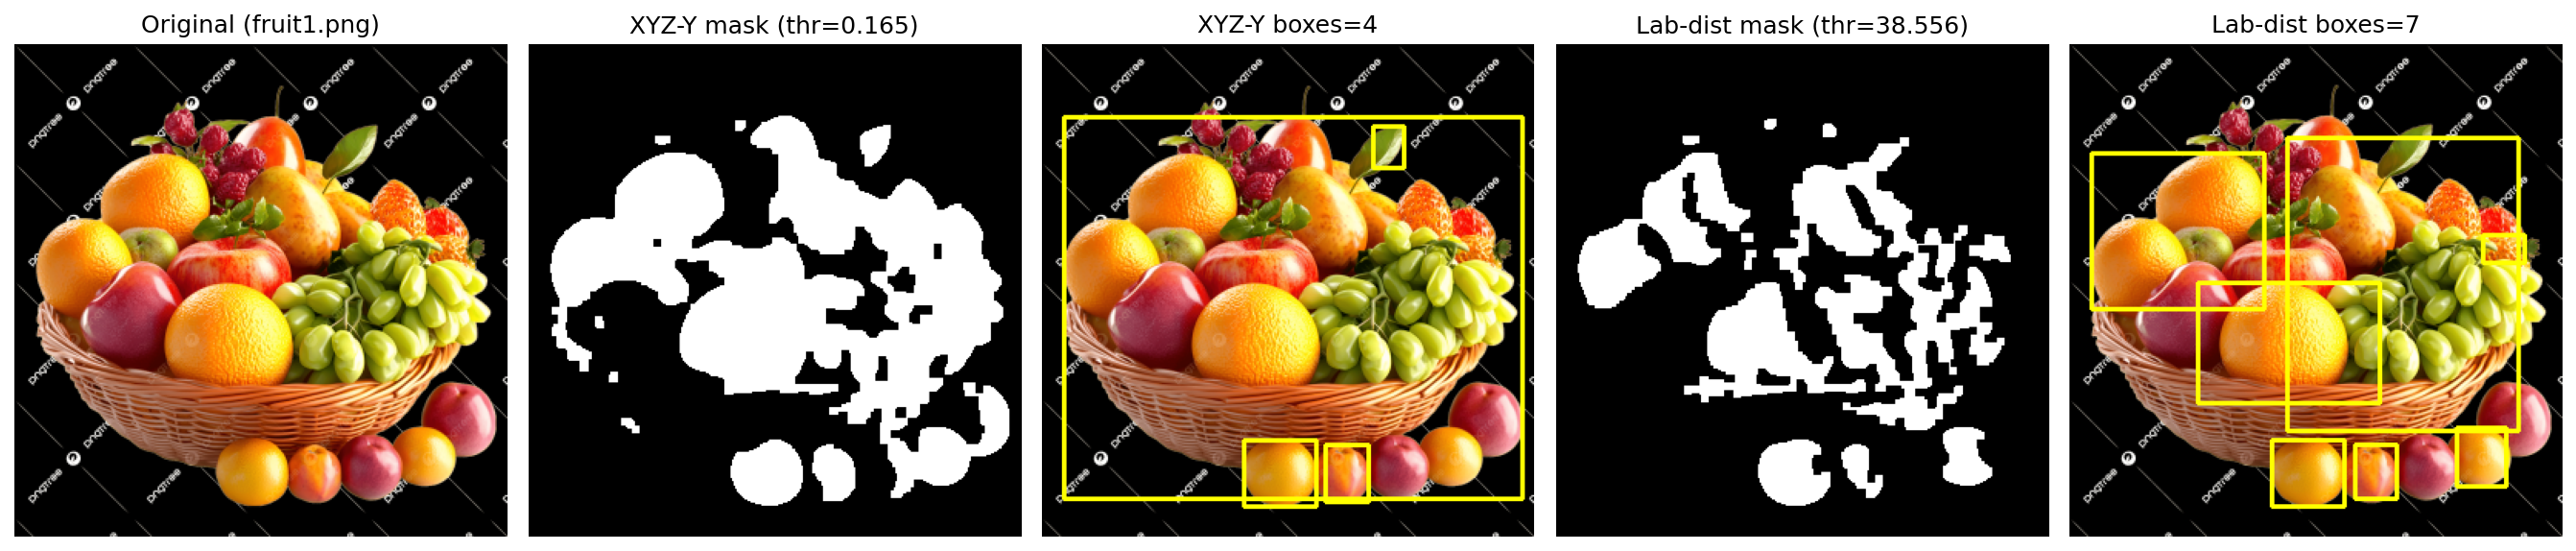
\includegraphics[width=\linewidth]{outputs/mini_project_fruit1_xyzY_vs_lab.png}
        \caption{fruit1.png}
    \end{subfigure}
    \hfill
    \begin{subfigure}{0.48\linewidth}
        \centering
        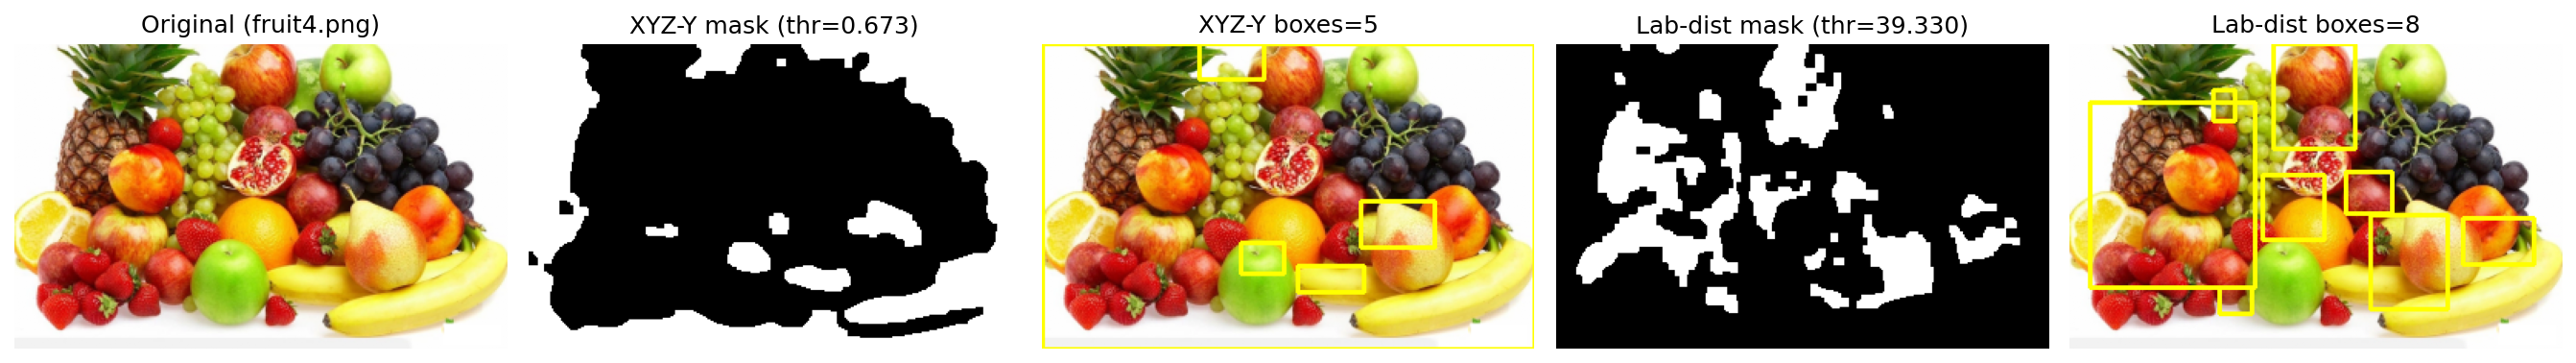
\includegraphics[width=\linewidth]{outputs/mini_project_fruit4_xyzY_vs_lab.png}
        \caption{fruit4.png}
    \end{subfigure}
    \caption{Hai ví dụ khó/thất bại tương đối của mini-project}
\end{figure}

\section{So sánh định lượng hai phương án mini-project}

\subsection{Thống kê trung bình trên 5 ảnh}
\begin{table}[H]
    \centering
    \caption{So sánh trung bình XYZ-$Y$ và Lab-distance}
    \begin{tabular}{lcc}
        \toprule
        Chỉ số & XYZ-$Y$ & Lab-distance \\
        \midrule
        Số box trung bình & 10.60 & 8.20 \\
        Mask ratio trung bình & 0.3412 & 0.1803 \\
        \bottomrule
    \end{tabular}
\end{table}

Trên tập mini-project hiện tại, Lab-distance giảm trung bình khoảng
$\frac{10.60-8.20}{10.60}\approx22.6\%$ số box so với XYZ-$Y$,
đồng thời cho mask gọn hơn đáng kể về diện tích.

\subsection{Ghi chú từ Bài toán 5 (K-means)}
Kết quả trung bình silhouette ở phần phân đoạn cho thấy
$\overline{s}_{XYZ}=0.5675$ và $\overline{s}_{Lab}=0.5191$ (với $K=4$),
nghĩa là không có một không gian màu luôn vượt trội trong mọi tác vụ.
Lợi thế của Lab trong báo cáo này nổi bật nhất ở bài toán phát hiện theo màu
dựa trên khoảng cách màu và hậu xử lý hình thái.

\section{Kết luận và hướng cải tiến}

\subsection{Kết luận}
Từ các thí nghiệm đã thực hiện:
\begin{itemize}
    \item Phần bắt buộc synthetic đã minh họa rõ failure modes của phương pháp dựa độ sáng
    và lợi thế của gradient màu trong XYZ/Lab.
    \item Trong mini-project phát hiện trái cây, Lab-distance cho kết quả sạch hơn ở đa số ảnh,
    thể hiện qua giảm số box trung bình và giảm mask ratio.
    \item Tuy vậy, vẫn tồn tại ca khó khi chọn màu mẫu chưa đại diện hoặc có vùng phản quang/bóng đổ mạnh.
\end{itemize}

\subsection{Hướng cải tiến}
\begin{enumerate}
    \item Dùng khoảng cách có trọng số:
    $d_w=\sqrt{w_L(L-L_0)^2+w_a(a-a_0)^2+w_b(b-b_0)^2}$ với $w_L<w_a,w_b$
    để giảm nhạy với biến thiên chiếu sáng.
    \item Kết hợp ngưỡng thích nghi theo từng ảnh thay vì quantile cố định.
    \item Hậu xử lý theo hình dạng (tỷ lệ khung bao, độ tròn) để giảm box nhiễu nhỏ.
\end{enumerate}

\end{document}
